%------------------------------------------------------------
%------------------------------------------------------------
\subsection{Entity model}
\label{sec:entity-model}
The entity model of a {\UTP} instance defines its schedule horizon, course structure and resources, as well as properties of entities and relational maps (see 
Figure~\ref{fig:utp-entity-model} for a sketch of the meta-model and Figure~\ref{fig:utp-rule-1} for a toy example).  
First, the entity model uses a time grid that decomposes into weeks, weekdays and daily slots. %, the number of which is instance-specific. 
Weeks share the same weekdays and weekdays the same daily slots. The latter make up 24 hours and have the same duration. %measured in minutes. 
Note that neither successive weeks nor successive weekdays are assumed to be consecutive. %and that Monday is the first weekday by convention. 
The schedule horizon is implicitly defined by the series of time slots mapping to week, weekday and daily slot combinations. Slots hence serve as time points to represent start and end times of course sessions and to measure session duration, travel time and any gap between sessions.

% % For one-column wide figures use
% \begin{figure}[h]
% % \includegraphics{utp-time-grid.eps}
% \caption{{\UTP} 3-layered time grid}
% \label{fig:utp-time-grid}
% \end{figure}

Courses have a tree-structure wherein each course (e.g., Algorithms) decomposes into parts (e.g., Lecture and Lab), parts into classes (e.g., lecture classes A and B), and classes into sessions (e.g., sessions 1 to 10 for each lecture class). Class sessions are the elementary tasks to schedule when solving a {\UTP} instance and the model fixes their number, duration and sequencing. First, the classes of a course part are decomposed into an identical number of sessions of equal duration, both constants being part-specific. Although this approach forbids classes using different session durations in a course part, 
%it %provides flexibility for handling sessions independently wrt. scheduling and resource allocation.
%Fixed decompositions also 
it is paramount to capture requirements that rely on clear-cut sessions (e.g., starting lab classes after 2 lecture sessions, synchronizing the 5th sessions of the lab classes for a joint examination). Second, the sessions of a class are ranked in the model and must be sequenced accordingly in any solution (session 1 before session 2 \ldots). Note that sessions are considered uninterruptible and, in particular, may not overlap two days. 

\begin{figure}[ht]
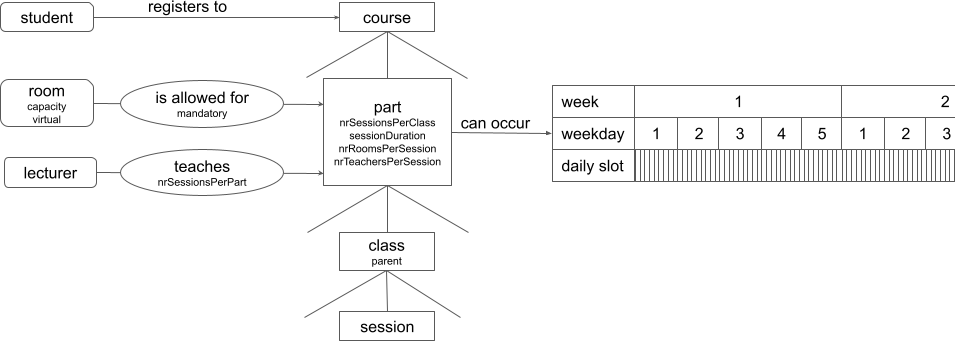
\includegraphics[scale=0.35]{img/utp_entity_model.png}
\caption{Entity meta-model.}
\label{fig:utp-entity-model}
\end{figure}

{\UTP} resources fall into 4 types, namely, rooms, lecturers, students and (student) groups.
All the resources of an instance, except groups (see Section~\ref{sec:solution}), are declared and typed in the entity model. In practice, upstream processes and decisions %constrain the resourcing and timing of courses.
%Basic restrictions come in the form of compatibility constraints that list 
determine the suitable rooms, eligible lecturers, candidate students and allowed times for the different courses (e.g., faculties prescribing degree-specific time grids, departments implementing room pooling policies and naming lecturers for courses, students registering to courses). %Such constraints are built in the entity model but scoped differently depending on resource types. %Specifically, 
These compatibility constraints are modeled by associating sets of possible start times, rooms and lecturers to each course part and a set of registered students to each course. Each session then inherits the sets of allowed resources from the course part and the course it belongs to.
%and which are implicitly the sessions.
%Student registrations are listed separately and %the possible students for a session are those registered to the course it sits in.
%any student registered to a course is considered a possible candidate for each of its sessions.

The entity model also encodes flow constraints that govern the distribution of resources over courses based on student registrations and capacity planning decisions (e.g., workload distribution between lecturers). First, each lecturer is allocated a fixed number of sessions in each course part he is eligible for, leaving lecturer-to-session assignment decisions to solvers. Second, each room allowed in a course part may be freely allocated to any session of the part (possibly none) but the model provides the flexibility to mark a room as mandatory in which case it will host or co-host all the sessions. As for students, the sectioning policy is implicit and complies with the course structure, i.e., each student must be assigned to a single class in each part of a course he has registered to and attend all sessions of these classes. In addition, the model supports group nesting constraints between classes to implement course-specific policies (e.g., aggregating student groups bottom-up from labs to lectures) or cross-course sectioning (e.g., imposing the same groups between classes of different courses of a curriculum).
 
Resource utilization is naturally subject to demand and capacity constraints.
Since modalities differ from one environment to the next, the language supports disjunctive and cumulative resources. The default policy is to consider all students, groups, lecturers and rooms as cumulative resources, i.e., they can attend, teach or host simultaneous sessions. Note though that rules may be stated to make some resources fully disjunctive or to prevent specific sessions from overlapping. Support for cumulative resources is paramount to address flexible attendance requirements (e.g., students assigned optional tutoring sessions that may overlap with compulsory courses) or to handle multi-class events (e.g., rooms hosting several classes for an exam or a conference). The model imposes no limits on the number of parallel sessions lecturers and students may attend. Rooms however may only host class sessions whose cumulated headcount is within their capacity. Upper bounds on room capacity and class size are encoded for all rooms and classes and the model also allows uncapacitated rooms to cater for the case of virtual rooms.

The language also supports sessions using multiple resources of the same type. %at any point in time.
The need for multiple rooms or lecturers arises in practical situations (e.g., multi-room sessions for hybrid teaching, joint supervision of practical work sessions, exams requiring several monitors). %and the number of resources required per session is course part dependent.
%such restrictions are expressed in the entity model through cardinality constraints. %that are lifted to course parts. 
To this end, the model associates to each course part the number of lecturers required per session 
and indicates whether the sessions are single- or multi-rooms.
Note that sessions without lecturers or rooms are allowed (e.g., unsupervised student project sessions).
The model enforces specific constraints to handle multi-room sessions which override the default room allocation policy. Specifically, students attending the session may be freely dispatched in rooms irrespectively of the group structure, the cumulated capacity of the allocated rooms is taken into account for hosting, uncapacitated rooms cannot be allocated, and 
the allocated rooms are considered disjunctive for the time of the session.
%a {\UTP} instance may freely mix single- and multi-resource sessions as well as disjunctive and cumulative resources. 

Note finally that the language provides users with the ability to label resources and course elements to define their own classes of entities (e.g., teams of lecturers, blocks of rooms). Labels together with built-in entity types and identifiers are used to filter entities and to scope rules appropriately.
 


We formalize below the entity model and introduce notations that will be used thereafter.
Let ${\ENTITY}$ denote the set of entities
and ${\SESSION}$ the set of sessions.
${\ENTITY}$ is partitioned into   
a set of courses ${\COURSE}$, 
a set of course parts ${\PART}$, 
a set of classes ${\CLASS}$, 
a set of students ${\STUDENT}$, 
a set of lecturers ${\TEACHER}$,
a set of rooms ${\ROOM}$,
and the singleton domain of courses ${\COURSES}$ 
(${\COURSES}=\myset{\COURSE}$). 
Let 
%${\COURSES}$ denote the course domain, 
%${\COURSE}$ the set of courses (${\COURSES}=\myset{\COURSE}$), 
%${\PART}$ the set of course parts, 
%${\CLASS}$ the set of classes, 
%${\SESSION}$ the set of sessions, 
%${\STUDENT}$ the set of students, 
%${\TEACHER}$ the set of teachers, 
%and 
%${\ROOM}$ the set of rooms.
$
{\TYPE}
=
\myset{
{\COURSES}, 
{\COURSE},
{\PART},
{\CLASS},
{\STUDENT},
{\TEACHER},
{\ROOM}
}
$
denote the set of entity types
(${\ENTITY}=\setunion{X}{\TYPE}{X}$)
and 
$
{\prec}
=
\myset{
({\COURSES},{\COURSE}),
({\COURSE},{\PART}),
({\PART},{\CLASS}),
({\CLASS},{\SESSION}),
({\STUDENT},{\COURSE}),
$
$
({\TEACHER},{\PART}),
({\ROOM},{\PART})
}
$
denote the relation over 
${\TYPE}\cup\myset{\SESSION}$ 
that models the course hierarchy
and the distribution of resource types over course components.

${\prec^{*}}$
%${\preceq^{*}}$
denotes the transitive %and reflexive 
closure of
${\prec}$ 
over
${\TYPE}\cup\myset{\SESSION}$
and
${\maptype{X}{Y}}:X\rightarrow2^{Y}$
denotes the function mapping each element of $X$ to its set of compatible elements in $Y$
for each pair %$(X,Y)$ such that 
%$X{\preceq^{*}}Y$.
$X{\prec^{*}}Y$.
For instance, 
${\maptype{\ROOM}{\PART}}$ 
represents the distribution of rooms over course parts, 
${\maptype{\PART}{\CLASS}}$ 
the decomposition of course parts into classes,
${\maptype{\CLASS}{\SESSION}}$ 
the decomposition of classes into sessions,
and ${\maptype{\ROOM}{\SESSION}}$ 
the inferred distribution of rooms over sessions.
The functions corresponding to the pairs of $\prec$
are directly encoded in the entity model
and the remaining functions are defined inductively using recursive aggregation. 

We shall denote by ${\map{X}{Y}{i}}$ the image of entity $i$ of type $X$ over $2^Y$ %, i.e., the set of elements of type $Y$ compatible with $i$. 
and by ${\maptype{Y}{X}}$ the inverse of ${\maptype{X}{Y}}$.
Equation (\ref{model:hierarchy}) below models the hierarchical decomposition of course elements\footnote{$\sqcup$ denotes the disjoint union operation, i.e. set union over pairwise disjoint sets.},
Equation (\ref{model:transitivity}) is the closure rule over 
%$\preceq^{*}$. 
$\prec^{*}$,
%Note that each map $\maptype{\SESSION}{X}$ is the inverse of map $\maptype{X}{\SESSION}$.
and Equation (\ref{model:inverse}) models inverse maps.

\begin{align}
%
\forall (X,Y) \in 
\myset{
({\COURSES},{\COURSE}),
({\COURSE},{\PART}),
({\PART},{\CLASS}),
({\CLASS},{\SESSION})
}:
Y=
\setpartition{i}{X}{\map{X}{Y}{i}} 
\label{model:hierarchy}
\\
%
\forall X,Y,Z \in {\TYPE}\cup\myset{\SESSION}:
X\preceq^{*} Y\preceq^{*} Z 
\Rightarrow 
(\forall i \in X:
\map{X}{Z}{i}=\setpartition{j}{\map{X}{Y}{i}}{\map{Y}{Z}{j}}
\label{model:transitivity})
\\
%
\forall X,Y \in {\TYPE}:
X\preceq^{*} Y 
\Rightarrow 
(\forall i \in X, j \in Y:
j \in \map{X}{Y}{i} \Leftrightarrow i \in \map{Y}{X}{j}
)
\label{model:inverse}
%\\
%%
%\forall X \in {\TYPE}\cup\myset{\SESSION},
%i \in X:
%\domarg{X}{X}{i} = \myset{i} \label{model:selfmap}
%%
\end{align}



\begin{table}[ht]
\begin{center}
\begin{tabular}{|rl|}
\hline
$(\WEEK,\WEEKDAY,\DAILYSLOT)$               & the number of weeks $\WEEK$, weekdays $\WEEKDAY$ and daily slots $\DAILYSLOT$
\\
$\SLOT$                                     & the time slots 
\\\hline
$\ENTITY$                                   & the entities
\\
$\COURSES\subseteq\ENTITY$                  & the course domain
\\
$\COURSE\subseteq\ENTITY$                   & the courses
\\
$\PART\subseteq\ENTITY$                     & the course parts
\\
$\CLASS\subseteq\ENTITY$                    & the classes
\\
$\ROOM\subseteq\ENTITY$                     & the rooms
\\
$\TEACHER\subseteq\ENTITY$                  & the lecturers
\\
$\STUDENT\subseteq\ENTITY$                  & the students
\\
$\map{X}{Y}{i}\subseteq{Y}$                 & the entities of type $Y$ associated with entity $i$ of type $X$
\\\hline
${\LABEL}\subseteq2^{{\ENTITY}}$            & the labels
\\\hline
$\GROUP\subseteq{2^{\STUDENT}}$             & the groups of students
\\\hline
$\SESSION$                                  & the sessions
\\
$\map{X}{\SESSION}{i}\subseteq{\SESSION}$   & the sessions compatible with entity $i$ of type $X$
\\
$\map{\SESSION}{X}{s}\subseteq{X}$          & the entities of type $X$ compatible with session $s$
%\\
%$\disjunctiverooms\subseteq{\ROOM}$         & the set of disjunctive rooms
\\
$\partallowedslots{s}\subseteq{\SLOT}$      & the start times allowed for session $s$
\\
$\sessionduration{s}\in{\SLOT}$             & the duration of session $s$
\\
$\sessionrank{s}\in{\NATURAL^*}$            & the rank of session $s$ in its class
\\
$\sessionranked\subseteq{\SESSION\times\SESSION}$ & the pairs of sessions with consecutive ranks in a class
\\\hline
$\classparents{k}\subseteq{\CLASS}$          & the parent classes of class $k$ if any
\\
$\classcapacity{k}\in{\NATURAL}$            & the maximum size of class $k$
\\\hline
$\roomcapacity{r}\in{\NATURAL}$             & the capacity of room $r$
\\
$\virtualroom{r}\in{\BOOLEAN}$              & whether room $r$ is virtual or not
\\
$\virtualrooms\subseteq{\ROOM}$             & the virtual rooms
\\\hline
$\multiroompart{p}\in{\BOOLEAN}$            & whether course part $p$ is multi-room or not
\\
$\multiroomparts\subseteq{\PART}$           & the multi-room parts
\\
$\mandatoryrooms{p}\subseteq{\ROOM}$        & the mandatory rooms of part $p$
\\
$\partteachermultiplicity{p}\in{\NATURAL}$  & the number of lecturers required by every session of part $p$
\\
$\partteacherservice{l,p}\in{\NATURAL}$     & the number of sessions required by lecturer $l$ in part $p$
\\
\hline
\end{tabular}
\caption{Entity model: constants, sets, maps and relations.}
\label{table:model-maps}
\end{center}
\end{table}


Table~\ref{table:model-maps} provides the full list of constants, sets, properties and relational maps encoded in the entity model.\footnote{
The following rules apply. $\SLOT=\myset{i.\WEEKDAY.\DAILYSLOT+j.\DAILYSLOT+k\ |\ 0\leq i<\WEEK,0\leq j<\WEEKDAY,1\leq k\leq\DAILYSLOT}$.
For each class $k$ in part $p$,
$\myset{\sessionrank{s}\ |\ s\in\map{\CLASS}{\SESSION}{k}}=\myset{1,\ldots,\mycard{\map{\CLASS}{\SESSION}{k}}}$, 
%$\mycard{\classparents{k}}\leq1$ 
and $\classparents{k}\not\subset\map{\PART}{\CLASS}{p}$.
For each pair of sessions $s,s'$, 
$(s,s')\in\sessionranked$ iff $\map{\SESSION}{\CLASS}{s}=\map{\SESSION}{\CLASS}{s'}$ and $\sessionrank{s'}=\sessionrank{s}+1$.
For each course part $p$,
%$p\in\multiroomparts$ iff $\multiroompart{p}$; 
%and 
$\partteachermultiplicity{p}.\mycard{\map{\PART}{\SESSION}{p}}=\sum\limits_{l\in\map{\PART}{\TEACHER}{p}}{\partteacherservice{l,p}}$.}

%We shall denote by
%${\RANK}$
%the range of session ranks,
%${\maptype{\RANK}{\SESSION}}:\RANK\rightarrow2{^\SESSION}$
%the rank-based partitioning of sessions,
%and
%${\LABEL}$
%the set of labels 
%(${\LABEL}\subseteq2^{{\ENTITY}}$)
%completed 
%with the whole set of entities %to mock label optionality
%($\ENTITY\in{\LABEL}$)
%and singleton entities %to support identity-based selection
%($\myset{\myset{e}\ |\ e\in{\ENTITY}}\subseteq{\LABEL}$).
%As discussed in section~\ref{sec:rules},
%labels are optional filters used in rules to select entities
%hence the formal inclusion of $\ENTITY$ in ${\LABEL}$ to mock label optionality.
%Likewise, entity identifiers are used as an alternative to labels
%hence the inclusion of singleton entities in ${\LABEL}$.
